\documentclass[12pt]{article}

%% - - - page formatting
% \renewcommand{\baselinestretch}{2.0}
\usepackage[doublespacing]{setspace}
\usepackage[margin=1in, left=1in, top = 1in, includefoot, a4paper]{geometry} 
\usepackage[document]{ragged2e}
\setlength{\RaggedRightParindent}{2em}
\RaggedRight
\usepackage{indentfirst}
\setlength\footnotemargin{0em}
\usepackage{appendix}
\usepackage{endnotes}
\renewcommand{\theendnote}{\Roman{endnote}} 
\usepackage{enumerate}
\usepackage{enumitem}

%% - - - Citations & References
\usepackage[style=apa,hyperref=true]{biblatex}
% \addbibresource{./references.bib}
\bibliography{./references.bib}

\usepackage{hyperref}
\hypersetup{
    colorlinks = true,
    urlcolor = blue,
    citecolor = [rgb]{0, .121, .388},
    linkcolor = [rgb]{.349, 0, 0},
}

% personal preference :)
\let\oldcite=\cite
\let\oldtextcite=\textcite
\renewcommand{\cite}[1]{\textcolor[rgb]{0, .121, .388}{\oldcite{#1}}}
\renewcommand{\textcite}[1]{\textcolor[rgb]{0, .121, .388}{\oldtextcite{#1}}}


%% - - -  Math
\usepackage{mathtools}
\usepackage{algorithm}
\usepackage{algorithmic}

%% - - - Media
\usepackage{graphicx}
\usepackage[rightcaption]{sidecap}

\pagenumbering{roman}



\title{Deep Neural Networks as End-To-End Models of Object Recognition}
\author{Matt Wetzel}


\begin{document}

% % % % % % % % % %
%
%   TITLE
%
% % % % % % % % % %
\maketitle
\pagebreak

\tableofcontents
\pagebreak




% - - - - - - - - - - - - - - - - - - - - - - - - - - - - - - - - - - - - - - - - - - - - - - - - - - - - - - - - - - - - - - - - - - - - - - - - - - - - - - - - - - - - - - - - - - - - - - - - - - - - - - - - - - - -





% % % % % % % % % %
%
%   CONTENT
%
% % % % % % % % % %

\section{Introduction}
\pagenumbering{arabic}


Deep learning models have recently experienced major success at solving a wide variety of computational challenges in the machine learning literature (\cite{lecun2015deep,he2015delving}), spanning domains like vision \& perception (\cite{lecun1995convolutional}), language (\cite{hochreiter1997long}), and reinforcement learning in less-structured environments (\cite{mnih2013playing}). Deep learning (and more generally, \emph{connectionism}) has also played an important role in theories of cognition across a number of different psychological literatures. In addition, many recent developments in deep learning research have been inspired by the animal brain (\cite{lecun2015deep,sabour2017dynamic,graves2014neural,jarrett2009best}). It is therefor unsurprising that researchers have begun exploring whether deep learning's modern instantiation has any utility as an explanatory model of human cognition (see \cite{yamins2016using,serre2019deep,storrs2019deep} for reviews). The goals of the present paper are to (1) address the recent successes and failures of deep learning in accounting for human object perception, and (2) highlight emerging research directions that might be promising in addressing its current limitations. The next section will provide a brief overview of connectionism \& deep learning, with a particular focus on variants that have received much attention in the perception literature.

\subsection{Deep Learning \& Connectionism}

In a foundational paper, \textcite{mcculloch1943logical} provided a mathematical description of neural communication as a logical circuit of interconnected processing units (or, \textbf{artificial neurons}). Since, researchers in both cognitive science and artificial intelligence have demonstrated that networks of interconnected, artificial neurons are capable of performing very difficult feats of cognitive behavior (\cite{schmidhuber2015deep}). Connectionism is the theoretical position that many facets of animal behavior emerge from the collective dynamics of neural networks (\cite{rumelhart1986general}), constrained by a restricted set of architectural and computational principles. In connectionist networks (figure \ref{fig:feedforward}), each neuron takes on some scalar value, referred to as its \textbf{activation}. Typically, a neuron's activation is modified by some nonlinear function, referred to as the \textbf{activation function} of the neuron. Information from the network's environment propagate through weighted connections between neurons, referred to as \textbf{synapses}. 

% standard ff connectionist model
\begin{figure}[!h]
    \centering
    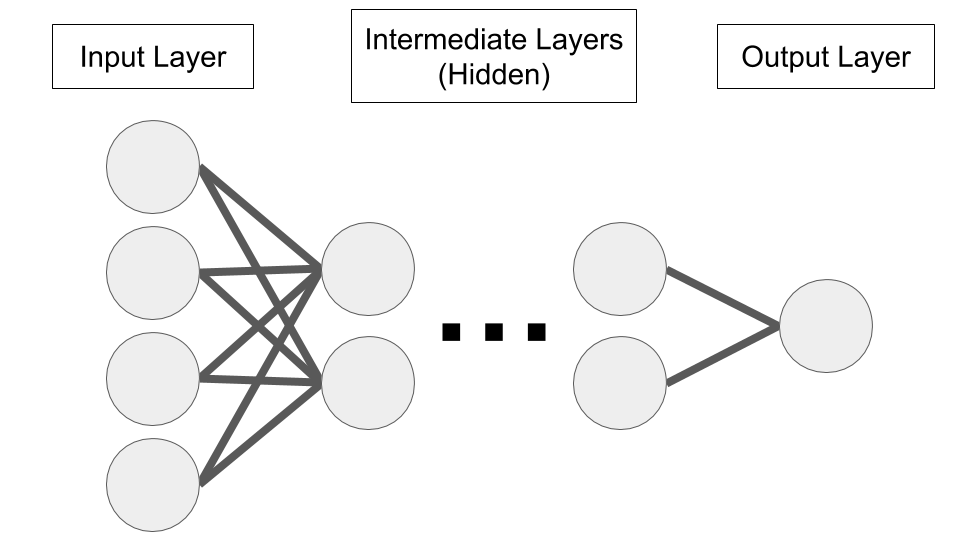
\includegraphics[scale=.4]{figures/feedforward.png}
    \caption{Example of a fully-connected, feedforward connectionist networks. The input layer represents data from the environment, which is propagated through a series of intermediate layers (also referred to as \emph{hidden layers}) before eventually reaching the output layer (which, after optimization, should produce some experimenter-defined ideal behavior). Note: not all connectionist models are feedforward (\cite{hinton2007boltzmann,kohonen2007kohonen,hopfield2007hopfield}).}
    \label{fig:feedforward}
\end{figure} 

Learning in a connectionist network typically involves updating the synaptic connections between nodes in a way that makes the network produce a desired behavior. The artificial network models proposed by early theorists were often very shallow, consisting of laminar-structured networks with only 1 sequence of connections between two layers of artificial neurons (e.g., input and output layers; \cite{rosenblatt1958perceptron,schmidhuber2015deep}). Soon after, many researchers began exploring the consequences of long chains of neural layers (i.e., \emph{deep learning}; \cite{ivakhnenko1965cybernetic,lecun1989backpropagation,lecun1995convolutional}), allowing networks to leverage compositionality in their representational structure. Additionally, researchers began integrating recurrency in the information propagation of relatively shallow architectures (\emph{recurrent neural networks}), allowing networks to capture temporal dependencies of sequential learning domains (\cite{jordan1990attractor,hochreiter1997long})\footnote{Interestingly, adding recurrency to neural networks gives them the expressive capability of general purpose computers (at least theoretically; \cite{schmidhuber2015deep}); see \textcite{graves2014neural} for an example of a memory-augmented recurrent network that learns a copy \& sort algorithm end-to-end via backpropagation. \\}. 

While there are many existing algorithms for updating the weights of an artificial neural network (\cite{tsodyks1989associative,stanley2002evolving}), many have argued that the recent success of deep learning has been driven primarily by the backpropagation algorithm (\cite{lecun2015deep,schmidhuber2015deep}). Backpropagation (\cite{kelley1960gradient,linnainmaa1976taylor,lecun1985procedure,rumelhart1986learning}) leverages the fact that information propagation in a neural network can be formalized as a chain of simple mathematical operations\footnote{mainly, addition and multiplication \\} (figure \ref{fig:activationFormula}). Using the chain rule, the weights of a neural network can be incrementally updated to optimize any desired output that can be measured via a mathematically tractable \textbf{cost function}\footnote{for example, the sum squared difference between a desired output vector and a target vector \\}. While the biological plausibility of backpropagation has been questioned (\cite{crick1989recent}; though see \cite{lillicrap2020backpropagation}), connectionist networks trained via backpropagation provide a compelling demonstration that a very simple credit assignment algorithm combined with a network architecture is capable of flexibly learning complex behaviors in both structured and unstructured environments\endnote{Backpropagation provides a way of updating the weights of a neural network throughout exposure to a training environment. However, the performance of a neural network is also sensitive to more macro-level properties, such as the architecture and weight update strength. These macro-level properties (known as \textbf{hyperparameters}) are not directly learnable via backpropagation, and are typically tuned by any class of gradient-free optimization algorithms (such as random searching, hill-climbing, or bayesian parameter estimation; \cite{bergstra2011algorithms}). Interestingly, \textcite{yamins2016using} make an interesting analogy between \emph{backpropagation::hyperparameter optimization} and \emph{synaptic plasticity::evolutionary selection}. The former (backpropagation \& synaptic plasticity) allow for flexible adaption to an organism's environment, while the latter (hyperparameter optimization \& evolutionary selection) can maximize the internal conditions necessary for online learning. Of further interest are the empirical demonstrations that genetic algorithms of evolutionary selection are quite useful for tuning the hyperparameters of large-scale connectionist networks (\cite{young2015optimizing,stanley2002evolving}). \\}. 

% formula of the activation of a neuron
\begin{figure}
    $$ a_h = \sigma(a_i \cdot w) $$
    \caption{Activity of a post-synaptic artificial neuron \(a_h\) can be described as the weighted sum of the activations of all incoming pre-synaptic neurons \(a_i\) (i.e., the matrix multiplication between pre-synaptic activations and weighted, synaptic connections \(w\)), transformed by some `activation function' \(\sigma\) (e.g., a \href{https://en.wikipedia.org/wiki/Sigmoid_function}{sigmoid function}). In a typical connectionist network, this step occurs for all neurons in all layers of the network. Backpropagation involves computing the derivative at each step in the chain of equations describing the entire network.}
    \label{fig:activationFormula}
\end{figure}


\paragraph{End-To-End Cognition}\mbox{} \\

End-to-end models of cognition describe learning throughout the entire behavioral pipeline of the organism being modeled (\cite{glasmachers2017limits}). Many theoretical branches within the categorization, relational reasoning, and causal learning literature have relied on experimenter-defined representations of the environment (\cite{nosofsky1994comparing,anderson1991adaptive,falkenhainer1989structure,hummel1996lisa,danks2014unifying}), as opposed to learning from raw perceptual data. As argued by \textcite{chalmers1992high}, this leaves many questions unanswered, including the question of how perceptual systems and cognitive reasoning systems interact. Connectionist models in cognitive psychology have also typically relied on hand-coded representations of the environment (\cite{rogers2004semantic,gluck1988conditioning,kurtz2007divergent}). However, the general structure of a connectionist network is readily adaptable to handle raw perceptual data; in fact, the success of connectionist architectures at handling perceptual data\footnote{As well as the advent of the GPU (\cite{schmidhuber2015deep}) \\} has been argued as a primary driver of the renewed interest in deep learning in both AI and cognitive psychology (\cite{lecun2015deep,schmidhuber2015deep}). This is particularly appealing in that it provides a mechanistic explanation of complex behavior (e.g., categorization, spatial relational reasoning, spatial navigation \& motor function) that starts at the level of sensation (i.e., \emph{end-to-end cognition}). 

\subsection{The Convolution Operation}

A standard, feed-forward connectionist network operates by propagating a numeric signal from the environment (i.e., information gathered from sensory \emph{nodes}) through a series of \emph{hidden} layers before eventually producing some target response at the \emph{output} layer. In a fully-connected network, a given neuron in the post-synaptic layer is connected to every neuron in the pre-synaptic layer. When applied to domains such as vision, each stimulus (or image) is represented in raw pixel values (loosely analogous to the tightly packed receptors in the retina). The value from each pixel is propagated through weighted connections in the network. Because images are composed of many pixels, training a fully-connected network on images is relatively inefficient, requiring exponentially more connections as the number of pixels increases. 

A breakthrough innovation in the deep learning literature was the use of the convolution operation (\cite{fukushima1983neocognitron,lecun1989backpropagation}). Rather than fully connecting a neuron to the entire pixel array of an image, a neuron in a convolutional neural network (CNN) contains a small set of weights applied to local patches sampled from an image (figure \ref{fig:forwardOperations}). This allows each neuron to act as a filter leveraging the statistical relationship between pixels that are close together in space\footnote{which is an important property of natural images: the spatial arrangement of pixels in an image is just as (if not more) predictive than each pixel value individually \\}. This hallmark step in the evolution of connectionist networks drew heavily on inspiration from classic findings in animal neuroscience (\cite{hubel1968receptive}), namely the hierarchical organization of laminar networks with spatially-tiled receptive fields. Modern CNNs also rely heavily on a biologically-inspired pooling operation (\cite{lecun2015deep}) that aggregates information from local patches of a convolutionally-transformed stimulus\footnote{though see \cite{springenberg2014striving} for an example of a CNN without an explicit pooling operation. \\}. Importantly, the convolutional and pooling operation leveraged by CNNs can be fluently integrated into any network architecture that starts with a continuous, perceptual stream of information with important spatial (or even temporal) dependencies\footnote{without heavily distorting any of connectionism's fundamental design principles \\} (e.g., images, videos, speech signals, pressure sensors, etc). 

% figure comparing normal representation of inputs in connectionist network on symbolic versus perceptual data
\begin{figure}[!h]
    \centering
    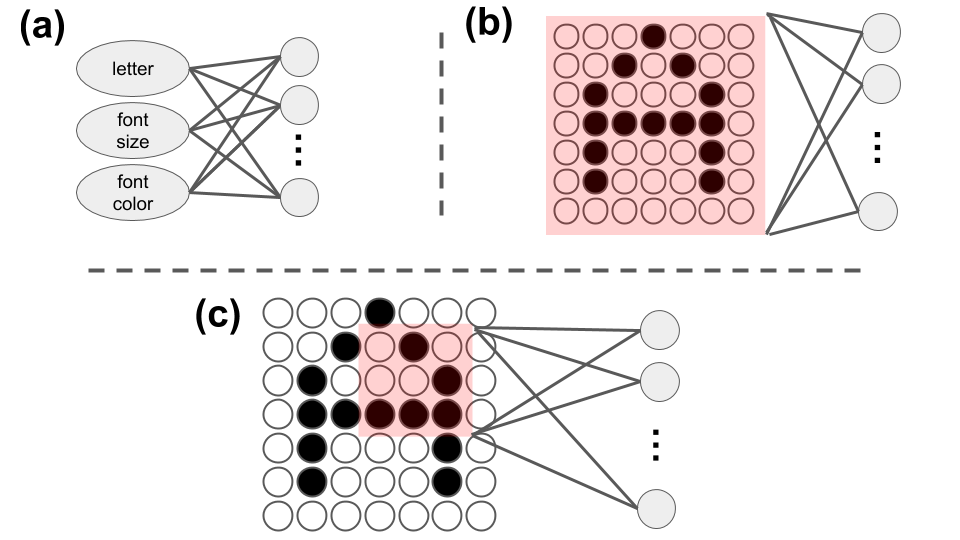
\includegraphics[scale=.4]{figures/forwardOperations.png}
    \caption{Comparison of different types of data representations and forward computations. }
        \begin{enumerate}[label=(\alph*)]
            \item A fully-connected layer representing an image based on it's symbolic, experimenter-defined features. 
            \item A fully-connected layer representing an image as an array of pixel values (each pixel shares a connection with each hidden node). 
            \item A convolutional layer, where images are represented as a pixel array, and a small receptive field connects each hidden layer to a local image patch. In a standard convolution operation, the local receptive field samples each region of the image, allowing CNNs to capture local patterns that are invariant to spatial location (i.e., translation-invariance).
        \end{enumerate}
    \label{fig:forwardOperations}
\end{figure} 

The unprecedented success of CNNs at visual recognition problems (as well as their explicit inspiration from animal neuroscience) has made deep learning an attractive framework for modeling end-to-end cognition in the animal brain; researchers have already used CNNs to make relatively plausible fits to a number of behavioral and physiological phenomena in the cognitive science literature (\cite{yamins2016using,storrs2019deep}). However, despite these early signs of success, many researchers have pointed out critical limitations in the explanatory power of CNNs and other deep learning models of cognitive behavior (\cite{serre2007feedforward,lake2017building,serre2019deep}). While many of these empirical demonstrations have relied on pre-trained CNNs originally designed for image classification competitions (\cite{simonyan2014very,krizhevsky2012imagenet,szegedy2015going}), there are some key design principles that highlight why CNNs (in any form) are unlikely to exhibit crucial elements of human perception (\cite{gulccehre2016knowledge}). The next sections will highlight the empirical successes and failures of CNNs at capturing behavioral phenomena, followed by a review of emerging developments that (the author argues) might address some of deep learning's present shortcomings as models of human cognition. 


% - - - - - - - - - - - - - - - - - - - - - - - - - -


\section{CNNs as Explanatory Models of End-to-End Perception}

\subsection{Potential Strengths}

A foundational finding in the animal perception literature was \textcite{hubel1962receptive}'s discovery that neurons in the early visual pathway fire preferentially in response to simple visual patterns, providing support for the notion that simple, local patterns could be aggregated hierarchically to allow neurons to capture increasingly complex patterns in natural scenes. Since \textcite{hubel1962receptive}'s original work, researchers have uncovered various visual patterns that elicit preferential firing of neurons spanning the visual pathway in both animals and humans (\cite{spillmann1987comparison,Alonso2009}). The idea of an increasingly complex visual hierarchy has been leveraged by a large number of computational models of the visual pathway (\cite{poggio2013models,fukushima1983neocognitron,lecun2015deep}). 

The discovery of translation-invariant neurons that select for specific visual patterns (such as direction and orientation) provided inspiration for the \emph{Neocognitron} (\cite{fukushima1983neocognitron}), which was the early predecessor to the modern CNN. By design, the hidden nodes of a convolutional network are each fed the pixel values of local patches of an image (analogous to receptive fields in animal neurons); transforming the pixel array before it reaches later layers. When trained via backpropagation, the hidden nodes of CNNs adapt to capture specific statistical patterns in a visual scene, with relatively more complex patterns being learned by the deeper layers of the network (\cite{lee2009convolutional}). Comparing the similarity between the preferential response patterns of neurons in CNNs and biological neural networks has provided one useful avenue for testing the psychological plausibility of CNNs as models of vision (\cite{yamins2016using}).

% figure of the hierarchy learned by Ng's DBNs

\paragraph{Predicting Neurophysiological Behavior}\mbox{} \\

An early demonstration by \textcite{linsker1988self} found evidence of orientation-selective hidden neurons in a sparsely connected network trained via a Hebbian-learning rule\footnote{Hebbian-learning has been suggested to be more biologically plausible than backpropagation (\cite{mazzoni1991more,xie2003equivalence}) \\} using white noise as network inputs. In another demonstration, \textcite{zipser1988back} trained a fully-connected 3 layer connectionist network (input\(\rightarrow\)hidden\(\rightarrow\)output) to learn an autoassociative mapping between retinal activity\footnote{represented similarly as a pixel matrix \\} and eye position coordinates. \textcite{zipser1988back} found that the activations of hidden neurons in the connectionist network closely resembled the receptive field patterns of neurons in the macaque area 7a\footnote{a region in the macaque parieto-visual area \\}. \textcite{lee2008sparse} trained a stacked Restricted Boltzman Machine\footnote{a type of generative, connectionist model \\} on natural image data, and found hidden layers' distributional response patterns were similar to neurons in macaque area V2\footnote{specifically, sensitively to complex shapes such as bars, angles, and arcs \\} (using data from \cite{ito2004representation}). While none of these demonstrations leveraged the convolutional operation (which has been foundational in getting connectionist models to achieve human-level performance on visual recognition tasks; \cite{he2015delving}), they laid the groundwork for comparative studies between performance-optimized\footnote{performance-optimized refers to the fact that the network was optimized to complete some top-level task, such as classification of natural images (\cite{yamins2014performance}) \\} deep learning models and neurons in the animal visual pathway.

In a recent demonstration, \textcite{cadena2019deep} found state-of-the-art predictions to the response patterns of macaque V1 neurons using a CNN pre-trained to classify natural images (specifically from the early-middle layers of a pre-trained network with 23 intermediate layers in total; \cite{simonyan2014very}). In a similar demonstration, \textcite{yamins2014performance} found that the mid-level layers of a performance-optimized CNN were highly predictive of individual neural responses to natural scenes in macaque V4, while the last layer was predictive of neural responses in IT (which is thought to represent category-specific visual information); importantly, the predictive success of CNNs in \textcite{yamins2014performance}'s experiment surpassed the prevailing computational accounts at the time (\cite{lowe2004distinctive,serre2007feedforward}). Interestingly, when searching for optimal CNN architectures, \textcite{yamins2014performance} found that classification accuracy was correlated with the network's ability to predict IT neural activity.

Another methodological approach for investigating the neurophysiological plausibility of deep learning models (as well as other computational frameworks) involves analysis of the pairwise similarity between models' and animals' responses to stimuli; or, \emph{Representational Similarity Analysis} (RSA; \cite{kriegeskorte2008representational}; figure \ref{fig:RSA}). The intuition behind RSA is: if the animal brain treats 2 stimuli as very dissimilar, then a psychologically realistic model of perception should treat those same 2 stimuli as very dissimilar as well (\cite{kietzmann2018deep}). An appealing aspect of RSA is that it allows for comparison between any detectable measures from animals (e.g., neural firing rates, EEG signals, fMRI responses, expressive behaviors) or models (e.g., layer activations of a CNN). Using RSA, \textcite{khaligh2014deep} found that final layers of a pre-trained CNN were highly predictive of both IT bold responses of human learners and IT single-cell recordings in macaques (again, outperforming existing frameworks). Using a similar preparation, \textcite{long2018mid} found that the intermediate layers (but not the earliest layers) of a CNN accurately predicted bold responses in human OCT (which is though to mediate high-level, visual representations of natural categories). 

% RSA, khaligh & kriegskorte, long et al
\begin{figure}[!h]
    \centering
    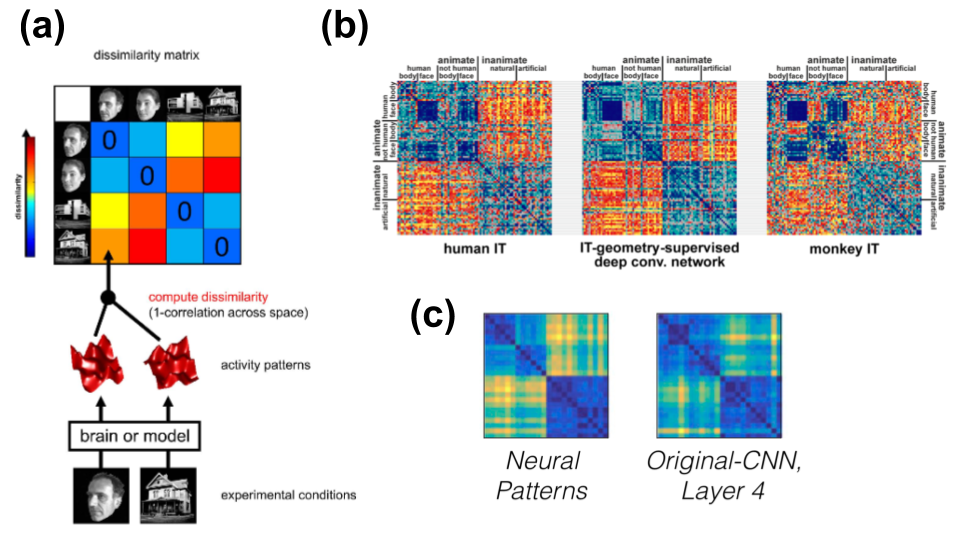
\includegraphics[scale=.4]{figures/RSA.png}
    \caption{}
        \begin{enumerate}[label=(\alph*)]
            \item Example of a hypothetical dissimilarity matrix used in RSA. Each cell in the matrix is computed by comparing the stimulus activations of some detectable measures, typically via a Pearson correlation (though see \cite{bobadilla2019measures} for an example of other similarity measures that can be useful). Taken directly from \textcite{kriegeskorte2008representational}. 
            \item Comparison of the dissimilarity matrices of human IT, monkey IT, and a modified CNN. Taken directly from \textcite{khaligh2014deep,kietzmann2018deep}. 
            \item Comparison of dissimilarity matrix of human OCT and the intermediate layer of a CNN pre-trained on natural images. Taken directly from \textcite{long2018mid}.
        \end{enumerate}
    \label{fig:RSA}
\end{figure} 

In summary, CNNs can be described as stacked layers of simple, interconnected artificial neurons that detect increasingly complex visual patterns (or features) from natural images. Further, the early layers of a CNN are predictive of the neural behavior of early layers of the animal visual stream (\cite{cadena2019deep,yamins2014performance}) while the later layers of a CNN are predictive of the later layers of the visual stream (\cite{khaligh2014deep,long2018mid}). Importantly, this explanatory success falls out of architectural insights about the animal perceptual system and a task-general learning algorithm designed to accomplish a behaviorally relevant goal --- \emph{not} via tuning the model's behavior towards neural behavior specifically. The success of backpropagation-trained CNNs in predicting neural behavior suggests preliminary evidence that animal neurons in the visual stream are adapted to meet the top-level behavioral demands imposed by an animal's environment. And, while the neurological plausibility of backpropagation has been questioned, it does seem to provide a way to tune artificial neurons in a way that's biologically consistent.

\paragraph{Predicting Cognitive Behaviors}\mbox{} \\

In addition to providing quantitatively accurate predictions of neurological data in primate brains (namely, humans and macaques), CNNs have also provided accurate accounts of a number of behavioral findings as well (\cite{lake2015deep,peterson2016adapting,dubey2015makes,kummerer2014deep}), using a variety of behavioral metrics. Pioneering work by \textcite{lake2015deep} found a correspondence between the classification decisions of pre-trained CNNs and the typicality judgments of natural images provided by human subjects, using a stimulus set of 8 categories each with 16 example images (e.g., bananas, bathtubs, mugs)\endnote{Predictive success of a model in \textcite{lake2015deep} was operationalized as the rank order correlation between mean human typicality ratings and the activation of the final classification layer of candidate CNNs.}. In addition to capturing the rank-ordering of human judgements, \textcite{lake2015deep} found that the activations of the latter layer of a CNN were \emph{more predictive} of typicality ratings than the early layers of a CNN, mirroring other empirical work suggesting that category-specificity emerges at the latter stages of the visual hierarchy in both the animal brain and CNNs (\cite{yamins2014performance,yamins2016using,khaligh2014deep,eickenberg2017seeing}).

% lake et al typicality figure
\begin{figure}[!h]
    \centering
    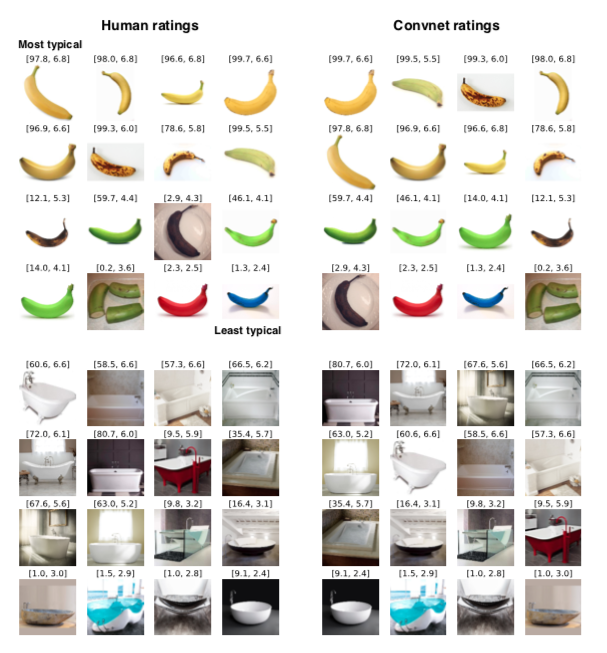
\includegraphics[scale=.7]{figures/lake2015deep.png}
    \caption{Typicality orderings (for images of bananas and bathtubs) of both human subjects and one of the candidate CNNs used in \textcite{lake2015deep} (the CNN used was the \emph{Overfeat} model; \cite{sermanet2013overfeat}). Figure taken directly from \textcite{lake2015deep}.}
    \label{fig:lake2015deep}
\end{figure} 

In addition to typicality judgments, the representations of CNNs have also been used to predict human \emph{similarity judgments} as well. Using a stimulus set of 120 natural images of animals, \textcite{peterson2016adapting} found --- using a metric similar to Representational Similarity Analysis (\cite{kriegeskorte2008representational}) --- that the penultimate\footnote{typically a fully-connected layer that precedes the final classification layer \\} layers of various pre-trained CNNs were moderately predictive of human similarity judgments of natural images (relative to low-level, category-agnostic image filters). In another demonstration, \textcite{dubey2015makes} trained human subjects to remember objects from a set of natural images, where each image contained a set of objects within it. \textcite{dubey2015makes} found that object memorability could be accurately predicted using feature representations of a CNN (at least, better than low-level image filters used in previous work; \cite{isola2013makes})\footnote{In addition, \textcite{dubey2015makes} found that the frequency of eye fixations was also predictive of object memorability/}.

Another empirical success of CNN models comes from their ability to predict eye
fixations of humans when viewing natural scenes (\cite{vig2014large,kummerer2014deep}). In one demonstration, \textcite{kummerer2014deep} found that a pre-trained CNN (Alexnet; \cite{krizhevsky2012imagenet}) achieved state-of-the-art performance at fitting the benchmark MIT300 saliency dataset (a database of fixations from 15 human subjects who observed a set of around 1000 images; \cite{judd2009learning}). \endnote{Saliency maps from Alexnet were generated by combining the filtered image representation of each feature map in a given layer (recall that each layer in a CNN contains a large set of feature maps)}. In addition to outperforming existing models at predicting human fixations, \textcite{kummerer2014deep} also found evidence of neurons in Alexnet that showed selectivity for faces, text, and even `pop-out' effects in natural scenes (figure \ref{fig:kummerer2014}). Importantly, this selectivity was an emergent property of a network trained to correctly classify images, rather than a design choice hand-engineered by an experimenter (as was the case for prior leading models of fixation prediction; \cite{judd2009learning}).

% figure kummerer2014deep
\begin{figure}[!h]
    \centering
    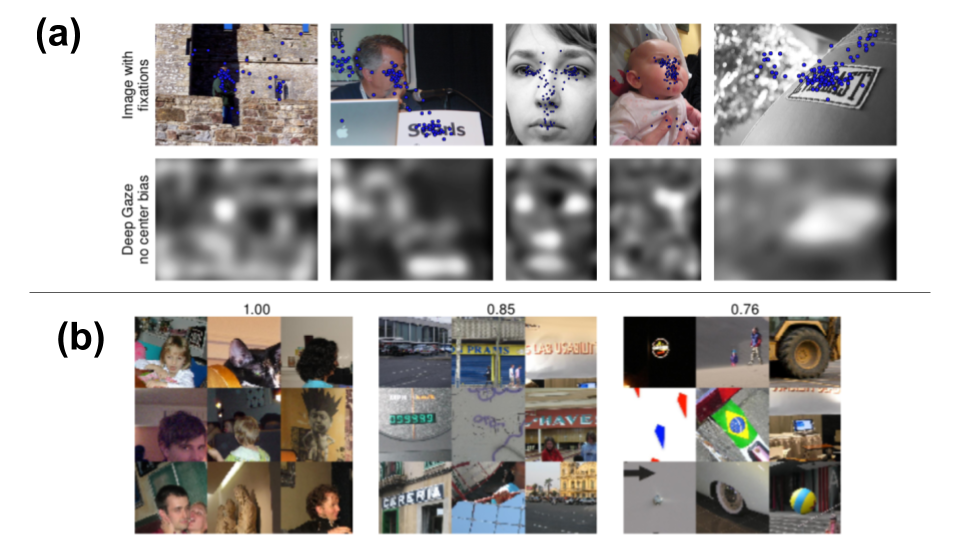
\includegraphics[scale=.4]{figures/kummerer2014.png}
    \caption{}
        \begin{enumerate}[label=(\alph*)]
            \item Top row: Example of the saliency map of human eye fixations from the MIT300 dataset (\cite{judd2009learning}). Bottom row: Results of \textcite{kummerer2014deep}'s method of generating saliency from CNN layers (more salient regions in white). 
            \item Example of images producing strongest activity from 3 selected neurons in \textcite{kummerer2014deep}'s analysis, highlighting sensitivity to different image features (e.g., faces, text, ``pop-out''). 
        \end{enumerate}
    Taken directly from \textcite{kummerer2014deep}.
    \label{fig:kummerer2014}
\end{figure} 

% plot of images that maximally activated the 3 most heavily weighted

\paragraph{Subsection Conclusion}\mbox{} \\

Work comparing CNNs to both neurological and behavioral phenomena is relatively new, but does provide preliminary support for CNNs as explanatory frameworks of \emph{some}\endnote{Note, the work discussed in this paper focuses on the \emph{what} pathway of perception (\cite{ungerleider2008and}), and does \emph{not} address the questions of how CNNs (and connectionism more broadly) handle other aspects of perception, such as object localization, navigation, and spatial reasoning (i.e., the \emph{where} pathway). See \textcite{grossberg2013adaptive} for a productive endeavor using neural networks to jointly model both the \emph{what} and \emph{where} facets of perception.} facets of animal perception. This tentatively suggests --- at the very least --- that the animal visual system is partly sensitive to some of the same visual statistics as CNNs. Despite being state-of-the-art, these results on their own aren't necessarily surprising, given that CNNs were inspired by the hierarchical, network structure of neural circuitry (\cite{mcculloch1943logical}) and the translation-invariance properties of some neurons in the visual stream (\cite{fukushima1983neocognitron}). Importantly, being a network hierarchy and translation-invariant are not the only core properties of animal vision. Namely, CNNs lack a practical level of viewpoint-invariance (\cite{sabour2017dynamic}), and don't take advantage of the object-centric, structured representations typically invoked in leading theories of animal perception (\cite{biederman1987recognition,tanaka1996inferotemporal,hinton1981shape}). These limitations may provide a critical roadblock in the explanatory power of CNNs, and may explain (in part) the empirical failures of CNNs described in the next section. 

\subsection{Potential Limitations}

\paragraph{Insensitivity to Global Object Shape}\mbox{} \\

Sensitivity to global shape is thought to be an important quality of human perception (\cite{biederman1987recognition,tanaka1996inferotemporal,hummel1992dynamic,biederman1993recognizing}), and the mechanisms of shape perception have been a productive explanatory challenge for cognitive psychologists. CNNs map objects to target behaviors by filtering images through a series of ``feature maps'' that are tiled along local patches of an image; this \emph{weight-sharing} procedure makes CNNs apt at capturing important, translation-invariant visual patterns that advance the immediate goal of image classification. However, the goal of image \emph{classification} does not necessarily require CNNs to gain object-centric image \emph{understanding}. That is, CNNs can form accurate mappings between images and class labels without accurately representing important object-part relationships. This has been referred to as the ``picasso problem''\footnote{in reference to Picasso's style of painting involving the rearrangement of object parts (figure \ref{fig:picassoProb}) \\}: CNNs recognition ability isn't particularly sensitive the global structure of an image defined by objects, object parts, and their relationships.\endnote{While it's less clear whether a CNN architecture can ever capture equivariant representations of global shape \emph{in theory}, they appear to functionally lack this property \emph{in practice}. \\}. While recent work (\cite{yamins2014performance,kietzmann2018deep}) has demonstrated that CNN representations accurately predict neural responses in the early visual stream (as well as behavioral judgments; \cite{peterson2016adapting,lake2015deep,kummerer2014deep}), other empirical work has demonstrated that CNNs fail to capture key, object-centric properties of human vision and visual reasoning (\cite{pramod2016computational,erdogan2017visual,baker2018deep}).

\begin{figure}[!h]
    \centering
    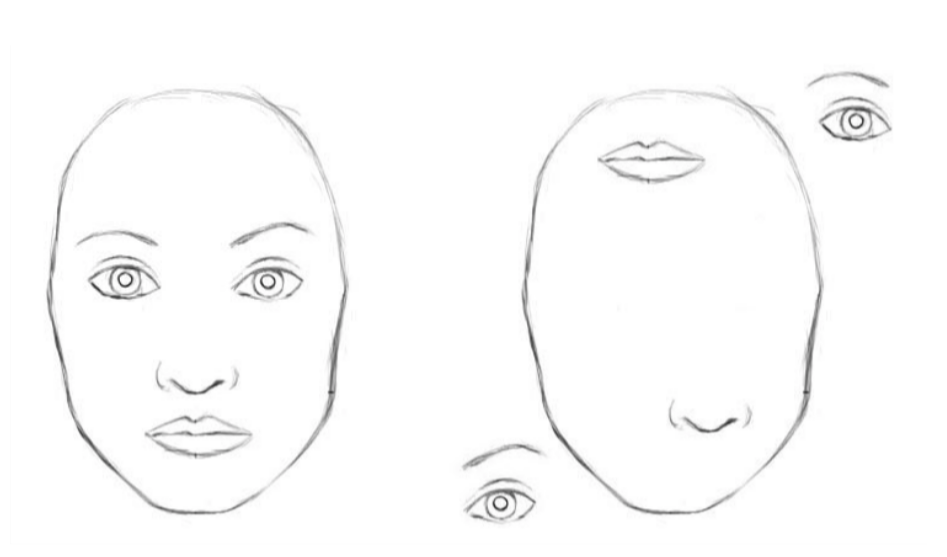
\includegraphics[scale=.4]{figures/picassoProb.png}
    \caption{Example of the Picasso problem: in practice, CNNs typically do not distinguish between either of the two faces, since they lack (in practice) a mechanism for capturing the spatial relationship between component features. Image taken directly from blog post by \href{https://medium.com/ai\%C2\%B3-theory-practice-business/understanding-hintons-capsule-networks-part-i-intuition-b4b559d1159b}{Max Pechyonkin}}
    \label{fig:picassoProb}
\end{figure} 

\begin{figure}[!h]
    \centering
    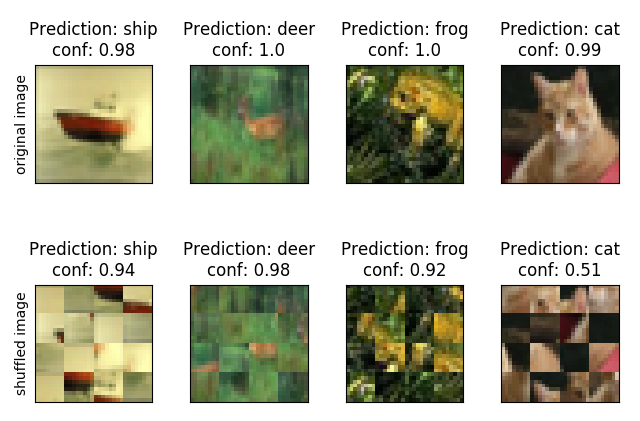
\includegraphics[scale=.7]{figures/googlenetFail.png}
    \caption{Example of a pre-trained CNN's (\cite{szegedy2015going}) response to 4 images taken from the CIFAR dataset (\cite{krizhevsky2009learning}). The CNN's predictions are qualitatively similar despite the images being shuffled in a way that distorts the spatial relationships between features, demonstrating the \emph{Picasso problem}.}
    \label{fig:googlenetFail}
\end{figure} 

In a large scale demonstration comparing 19 different models of the animal
visual system (including CNNs), \textcite{pramod2016computational} found that
CNNs (as well as other models) underplayed the importance of symmetry, spatial
area, shared object parts, and viewpoint in human dissimilarity perception using a database of ~26,000 dissimilarity measurements\footnote{Human dissimilarity was operationalized using the time it took to detect an object using a  preparation closely resembling a singleton detection task. \\} involving ~2,800 different object images. In another demonstration, \textcite{erdogan2017visual} had subjects judge the similarity between sets of procedurally-generated 3D objects that were either rotated, ablated, or reconfigured to some degree. While the similarity judgments from pre-trained CNNs\footnote{Similarity for CNNs was operationalized as the distance between stimulus-evoked activity vectors of a given CNN layer; CNN layers were from Alexnet (\cite{krizhevsky2012imagenet}) and GoogLeNet (\cite{szegedy2015going}) \\} were more similar to human judgments than other existing models of shape perception (\cite{poggio1990network,ullman1989aligning,riesenhuber1999hierarchical,feldman2013integrated}), \textcite{erdogan2017visual} found the strongest behavioral fit from their own model that leveraged Bayesian inference on structural, graph-based descriptions of stimuli (which is something CNNs arguably lack, at least in practice)\endnote{In an earlier demonstration of their work, \textcite{erdogan20163d} interpret their findings as evidence that CNNs are a fruitless modeling direction for explaining not only shape perception, but human vision in it's entirety, specifically citing CNN's focus on object categorization. Importantly, the convolutional operation is task-independent, and can be leveraged for both generative and discriminative learning objectives. Per \textcite{erdogan20163d} reasoning, a generative instantiation of a convolution architecture (\cite{lee2009convolutional}) may provide a more productive avenue for researchers than the standard, discriminative CNN models that are typically leveraged in cognitive neuroscience demonstrations (see \cite{yildirim2015efficient} for progress in this direction). Additionally, unlike the Bayesian inference model used by \textcite{erdogan2017visual}, CNNs are only provided with raw images as input, which is an arguably important constraint (\cite{yamins2016using}) on any model of animal vision that \textcite{erdogan2017visual} circumvent by using structured descriptions of objects rather than images. Nevertheless, \textcite{erdogan2017visual}'s work provides support for the theoretical view that structural descriptions are important for models of vision and shape perception (\cite{biederman1987recognition,griffiths2010probabilistic}). Though importantly, recent work has demonstrated that connectionist architectures provide a mechanism for learning structural models of visual scenes from raw sensory data. \\}.

\paragraph{Texture, Context, \& Adversarial Examples}\mbox{} \\

In a more direct investigation of CNN's ability to represent global shape, \textcite{baker2018deep} tested pre-trained CNN's generalization on images of unnatural instantiations of natural objects, as well as natural objects that were perturbed in some way. For example, some of the natural objects were depicted using the texture of a different object category. In other cases, objects consisted of black outlines against a white background \footnote{\textcite{baker2018deep} even included images of glass sculptures of natural images}. Importantly, these images and perturbations were designed in a way that shouldn't (intuitively) impede a human observers ability to classify the presented object (or any theoretical observer that's sensitive to global shape). Critically, \textcite{baker2018deep} found that two pre-trained CNNs (which previously achieved impressive performance on the ImageNet challenge; \cite{deng2009imagenet}) failed to appropriately classify a majority of the presented images. Interestingly, the two CNNs did seem to retain their ability to classify black, filled-in silhouettes of objects. As a result, \textcite{baker2018deep} hypothesized that the CNNs might capturing local shape statistics along the boundaries of objects. Consistent with this hypothesis, \textcite{baker2018deep} found that a slight perturbation to the outline of the silhouettes (figure \ref{fig:cnnFails}) greatly reduced the CNNs' accuracy at predicting object categories. In a similar demonstration, \textcite{geirhos2018imagenet} found that pre-trained CNNs could be easily fooled by swapping the the texture of one object with the texture of another (figure \ref{fig:cnnFails}). Further, \textcite{geirhos2018imagenet} demonstrated that instantiations of CNNs with higher degrees of shape bias were more resilient to image distortions than standard models.

\begin{figure}[!h]
    \centering
    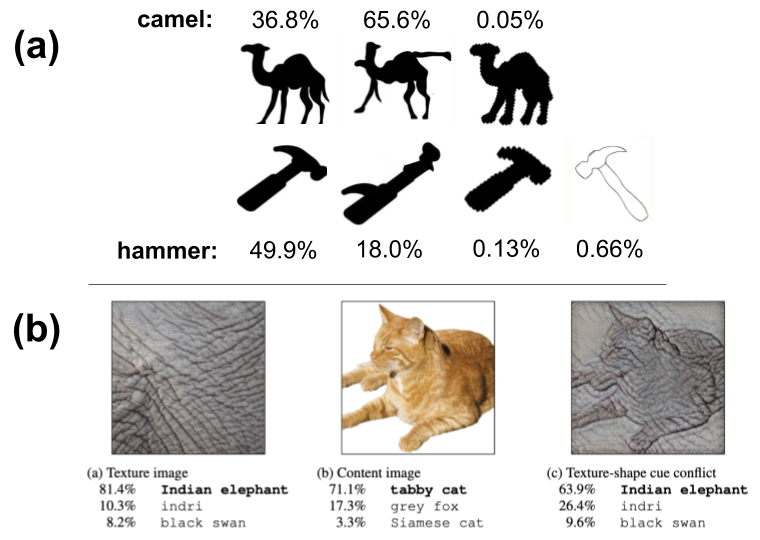
\includegraphics[scale=.45]{figures/cnnFails.png}
    \caption{}
        \begin{enumerate}[label=(\alph*)]
            \item Examples of distorted stimuli from \textcite{baker2018deep}, showing class predictions for original images and their distortions. In addition to generally lower performance for silhouettes (column 1), pre-trained CNNs generally seem insensitive to spatial feature relationships (column 2), and very sensitive to local edge information (column 3). Adapted from \textcite{baker2018contour}. 
            \item Example of images with swapped textures from \textcite{geirhos2018imagenet}, highlighting CNN's sensitivity to surface-level visual statistics. Taken directly from \textcite{geirhos2018imagenet}.
        \end{enumerate}
    \label{fig:cnnFails}
\end{figure} 


Another important limitation of CNNs stems from their limited ability to generalize to novel visual contexts. This was demonstrated by \textcite{rosenfeld2018elephant}, who found that object-detection systems that leverage CNNs often failed to identify (or instead misidentified) objects that were placed in an unlikely context (such as an inappropriately sized elephant in a hotel room; figure \ref{fig:rosenfeld2018elephant})\footnote{The debilitating context-sensitivity evident from \textcite{rosenfeld2018elephant}'s results might suggest that CNNs lack figure-ground distinction, which --- as argued by \textcite{serre2019deep} --- is a considerable explanatory shortcoming. \\}. While it's theoretically reasonable that humans might leverage textures and scenes to constrain their ability to correctly classify objects and events, the strength of this bias in pre-trained CNNs can greatly hinder their ability to generalize.

\begin{figure}[!h]
    \centering
    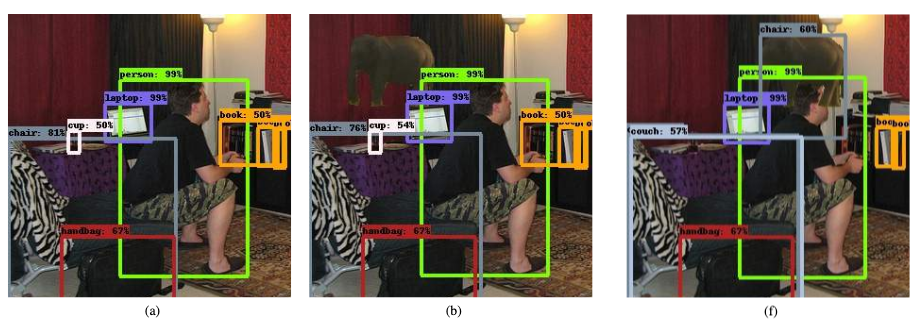
\includegraphics[scale=.4]{figures/rosenfeld2018elephant.png}
    \caption{Example of predictions from \textcite{rosenfeld2018elephant}. (a) shows the original image with object class predictions; (b) shows the network failing to classify the elephant in the room; (f) shows the network misclassifying the elephant as a chair, with relatively high confidence. Taken from \textcite{rosenfeld2018elephant}.}
    \label{fig:rosenfeld2018elephant}
\end{figure} 

In other demonstrations, researchers have found that the performance of CNNs can be greatly reduce by adding visual noise to images that would be otherwise negligible to the recognition accuracy of a human observer (\cite{jo2017measuring,geirhos2018imagenet}). Researchers have also uncovered various methods of producing stimuli that are unrecognizable to human observers while also eliciting high-confidence predictions from CNNs (known as \emph{adversarial examples}; \cite{nguyen2015deep,szegedy2013intriguing,goodfellow2014explaining}; figure \ref{fig:advEx}). Even further, \textcite{zhang2016understanding} demonstrated that CNNs could achieve high accuracy on a natural image dataset where the true labels of images are randomly shuffled. This raises long-term concerns about the falsifiability of deep learning models of vision, given that they are clearly flexible enough to utilize whatever image statistics (including noise) that are available in a given domain (independent of whether those image statistics are psychologically plausible). 

\begin{figure}[!h]
    \centering
    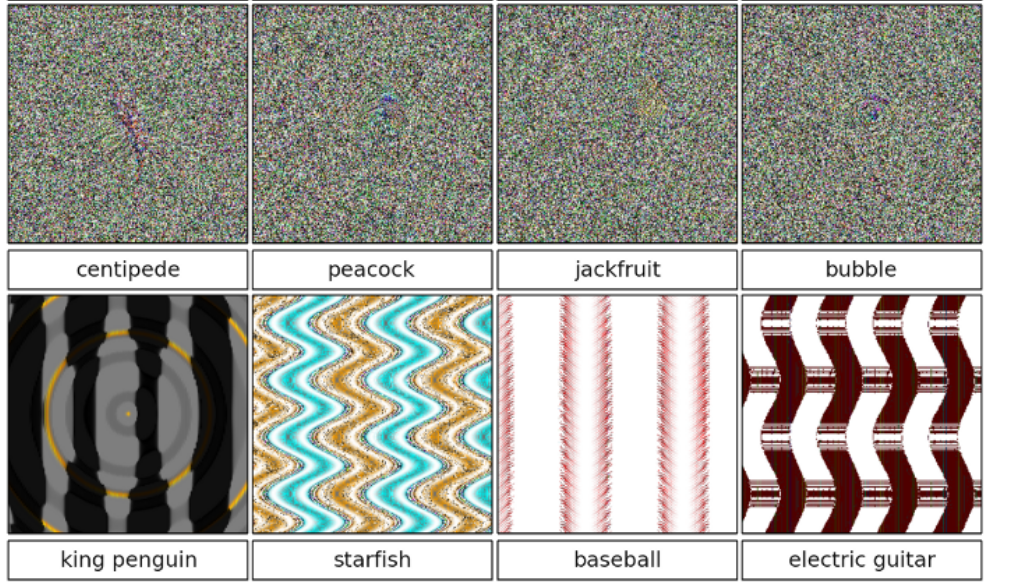
\includegraphics[scale=.4]{figures/advEx.png}
    \caption{Adversarial examples that illicit relatively confident predictions from models, while being unrecognizable by human observers. Take directly from \cite{nguyen2015deep}.}
    \label{fig:advEx}
\end{figure} 

\paragraph{Lack of Visual Reasoning Ability}\mbox{} \\

Being able to perform high-level reasoning on perceptual scenes is another hallmark behavior of human vision that popular variants of CNNs fail to achieve (\cite{serre2019deep,gulccehre2016knowledge}). One particular benchmark problem comes from \textcite{fleuret2011comparing}, who designed a Synthetic Visual Reasoning Test (SVRT) involving randomly generated images defined by an abstract rule or principle (figure \ref{fig:abstractProbs}a). Importantly, the images in the SVRT lack any complicated image statistics that could be leveraged by the feature maps of a CNN. \textcite{stabinger201625} found that 2 popular CNN architectures (\cite{lecun1989backpropagation,szegedy2015going}) were unable to learn to classify problems that required explicit comparison of objects in each image. Similarly, \textcite{gulccehre2016knowledge} found that CNNs (as well as other, distinct families of algorithms) are unable to generalize image categories defined by same-difference relationships between objects (\ref{fig:abstractProbs}b). While the failure of CNNs to handle these problems isn't necessarily surprising, the ease at which humans can solve abstract reasoning problems in visual scenes (\cite{fleuret2011comparing}) provide an important challenge for any end-to-end computational explanation of human cognition.

\begin{figure}[!h]
    \centering
    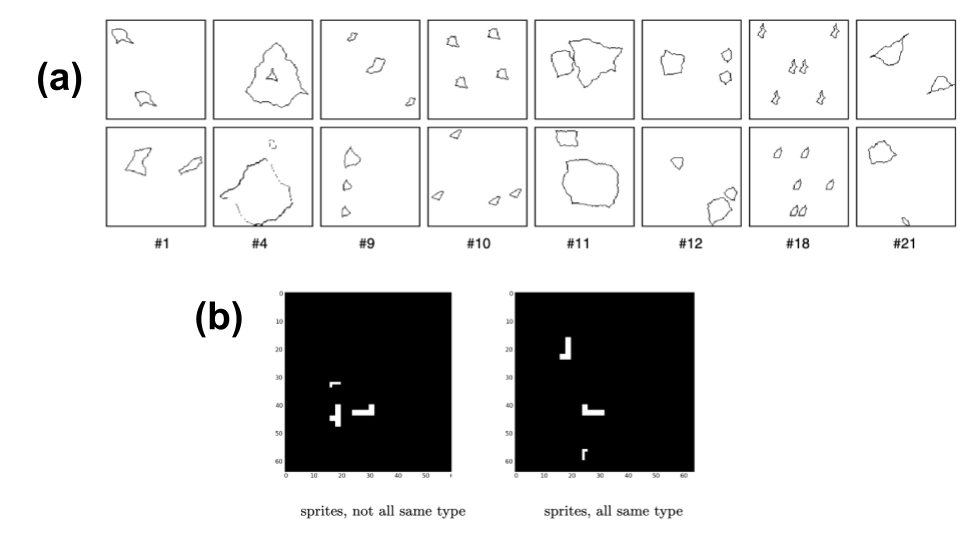
\includegraphics[scale=.4]{figures/abstractProbs.png}
    \caption{}
        \begin{enumerate}[label=(\alph*)]
            \item Example of SVRT image categories defined by abstract rules. Each column shows a different abstract category; each row is an example from one of the 2 categories for each concept. From \textcite{fleuret2011comparing}. 
            \item Example of same-different image categories, taken from \textcite{gulccehre2016knowledge}.
        \end{enumerate}
    \label{fig:abstractProbs}
\end{figure} 

\paragraph{Subsection Conclusion}\mbox{} \\

The previous section demonstrates areas where CNNs produce subpar performance at predicting a number of benchmark psychological phenomena, including key elements of global shape perception (\cite{baker2018deep}), contour detection (\cite{baker2018contour}\footnote{Though, see \cite{yang2016object} for advancements in this domain. \\}), and human-like generalization to new contexts (\cite{rosenfeld2018elephant}) or rotations (\cite{erdogan2017visual}; though see \cite{kheradpisheh2016humans}). In addition, feed-forward CNNs seem to lack any ability to perform abstract visual reasoning. On the one hand, these serious limitations might suggest a long-term weakness in using deep learning models to study end-to-end visual perception. On the other hand, CNNs have become state-of-the-art models for predicting human neurophysiological data as well as some elements of cognitive behavior in natural image domains. Further, many of the empirical limitations (and even successes) of CNNs are found in domains that CNNs weren't necessarily designed to accomplish (e.g., object-centric vision, abstract visual reasoning, fixations). The next subsection will provide some interpretation of these conflicting research findings.

\subsection{Synthesizing Conflicting Research Findings}

The convolutional operation allows connectionist networks to leverage a reduced
set of parameters (weights) to capture statistical patterns at local
regions across a visual scene (i.e., weight-sharing \& translation-invariance). Importantly, convolutional layers can be stacked, allowing later layers to take advantage of the statistical patterns captured by of the earlier layers (i.e., compositionality). Further, the statistical patterns captured at each layer are driven by the top-level goal of the model, which is typically classification. These are arguably the key properties that have resulted in CNNs unprecedented success at predicting behavioral and physiological phenomena of human and animal perception. That is, the visual path way of both CNNs and animals seem to utilize compositional, increasingly complex representations --- with category-specific differentiation emerging at the later stages. However, CNNs appear to be insensitive to the global shape of objects in a visual scene, and seem completely incapable of demonstrating any form of relatively simple visual reasoning\footnote{relative to humans \\}.

One interpretation of the successes and failures of CNNs naturally follows
Ramachandran's notion that ``vision is a bag of tricks'' (\cite{ramachandran1985neurobiology}); or in other words, the visual system is able to leverage \emph{any} arbitrary visual patterns that help solve some task. In the case of classification, the textures of a visual scene may be very useful for rapid, object classification (\cite{serre2007feedforward,rousselet2005long,loschky2010natural}). Object localization and figure-ground distinctions (core features of human perception that CNNs seemingly lack) might be orthogonal to the variance in physiological data that CNNs are adept at predicting. This idea is further supported by research demonstrating that humans can correctly recognize very broad categories of visual scenes after very brief exposure, even when attempts are made to reduce the degree of top-down processing after stimulus exposure (\cite{serre2007feedforward}). This might be the key relationship between CNNs and the animal visual system (at least in regard to the ventral stream): the proportion of variance in physiological and behavior data captured by CNNs might reflect the variance resulting from the initial, feed-forward sweep during early visual processing before any computations for object localization / figure-ground distinction have progressed. Given that the image statistics leveraged by CNNs are extremely useful for classification (evident by CNNs state-of-the-art classification accuracy on natural image datasets), it seems plausible that the human visual system might be sensitive to these same statistics as well (assuming that classification of broad-level image categories are particularly useful to a human's fitness). 

Even if the convolutional operation is orthogonal to the computations involved in object-centric perceptual processes, the representations learned by CNNs might be useful for object perception in important ways. For instance, if object and shape perception in humans is achieved through probablistic computations (as suggested by \cite{erdogan2017visual}), then category-specific representations might be particularly useful in constraining the appropriate hypothesis space the observer needs to search over, even if those category-specific representations are naive to global shape (as appears to be the case with CNNs; \cite{baker2018deep}). On the other hand, an additional (but not mutually exclusive) interpretation is that the convolutional operation lays the ground work for more complex perceptual computations by filtering visual information in a way that makes object perception easier. This naturally fits into some existing theories of object perception. For example, \textcite{biederman1987recognition}'s \emph{Recognition by Components} theory (RBC) posits that the first step in object perception is extracting edge information from a scene, followed by extraction of ``Nonaccidental Properties'' (e.g., curves, angles, verticies). The early layers of CNNs have been proposed to accomplish something akin to these first two stages of RBC. For example, \textcite{lee2009convolutional} found that the feature maps in the first layer of a generative convolutional deep belief net seemed useful for detecting edges, while the second layer seemed useful for detecting contours, angles, and corners (arguably similar to the \emph{vertices} invoked by RBC; figure \ref{fig:CNNs_doing_rbc}).

\begin{figure}[!h]
    \centering
    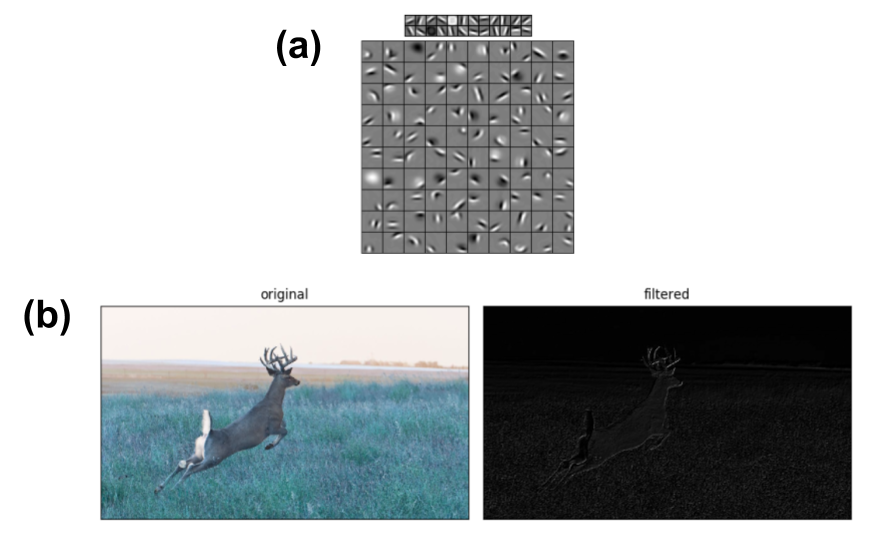
\includegraphics[scale=.4]{figures/CNNs_doing_rbc.png}
    \caption{}
        \begin{enumerate}[label=(\alph*)]
            \item Examples of feature detectors of a convolutional deep belief network, taken directly from \textcite{lee2009convolutional}. 
            \item Example of an image filtered through a randomly selected low level feature map of AlexNet (\cite{krizhevsky2012imagenet}). The resulting filtered image seems to perform some sort of edge extraction, the first stage of \textcite{biederman1987recognition}'s \emph{Recognition by Components} theory of object recognition.
        \end{enumerate}
    \label{fig:CNNs_doing_rbc}
\end{figure} 

Critically, this suggests that the early stages proposed by RBC can emerge
naturally from a network-structured learning algorithm that is task-optimized
via a universal learning rule. If this interpretation is accurate, it suggests
that CNNs might be psychologically realistic models of the early stages of
object-centric perception, and that the key explanatory roadblock might lie in
what happens \emph{after} edges and non-accidental properties have been
extracted. CNNs also share another key similarity with RBC: compositionality.
The featural information learned by a CNNs early layers are combined to form a
complex hierarchy of representations of a visual scene, seemingly analogous to
the \emph{geon} hierarchy proposed by RBC. The crucial difference (and arguably
the empirical limitations of CNNs as psychological models) is that the hierarchy learned by CNNs doesn't appear to be explicitly sensitive to global shape or the figure/ground distinction. It is an open question whether the convolutional operation can be leveraged to accomplish this (via regularization or a fine-tuned training procedure), or whether an entirely new computation is required (\cite{hinton2011transforming,sabour2017dynamic}).


% - - - - - - - - - - - - - - - - - - - - - - - - - -


\section{Future Directions in Deep Learning Research}

The previous sections have covered the successes and failures of CNNs as
explanatory models of human and animal perception. To review: CNNs seem to capture a significant portion of the variance in physiological and behavioral responses in both humans and animals across the ventral stream. However, the family of CNN models investigated in the literature seem to be insensitive to global shape, and seem to lack the ability to perform simple, visual reasoning tasks. A straightforward interpretation is that CNNs trained via backpropagation are leveraging statistical patterns in visual scenes similar to the patterns leveraged by the ventral stream; these visual statistics may be the key precursors to object-centric vision, or just useful ``tricks'' used to improve classification\footnote{or additionally, to constrain the hypothesis space of probabilistic mechanisms of shape perception \\}. However, any interpretation of the existing literature should warrant caution for a number of reasons.

First, CNNs are a very broad, flexible family of computational models (\cite{yamins2016using}); there are a number of architectural and mechanistic hyperparameters that influence a particular CNN's behavior\footnote{Importantly, this can be seen as a critical limitation: if CNNs are flexible enough to fit any behavior, they lose falsifiability and explanatory power as theoretical models of human perception. \\}. As a result, it's unclear whether the existing empirical successes and failures of CNNs reflect the convolutional operation itself, or just nuances of the models tested in the literature. Additionally, many of the CNNs leveraged in the literature underwent a very unnatural training experience: each time step in the training experience of CNNs typically involves random presentation of natural images from vastly distinct image categories (unlike the typical visual experience of a human learner). Further, CNNs are typically optimized for the goal of classifying broad-level categories of (often cluttered) 2 dimensional images; which deviates from the rich structure and perceptual constraints of normal visual experience (e.g., presence of motion, relative stability of the visual landscape, shape-centric learning objectives)\footnote{However, the use of pre-trained architectures is reasonable given that large-scale CNNs take a very long time to optimize and require an expensive amount of computational resources. \\}. The next section will highlight recent or promising advancements in the deep learning literature that help address the limitations of existing comparative studies. Additionally, novel advancements that address the issue of object-centric perception and visual reasoning will be discussed.

\subsection{Modifying the Learning Experience}

During each optimization step, CNNs are typically shown a sample of natural images from different broad-level categories (e.g., dog, cat, plane, etc). Importantly, this visual exposure is vastly different from the perceptual cirriculumn experienced by a human observer. A clever advancement in the developmental perception literature has leveraged head-mounted cameras and eye trackers worn in ``everyday'' environments to investigate the sequence and distribution of visual information experienced by infants interacting with their environment (\cite{smith2018developing,james2014some,james2014young}). Various work has illuminated important biases\footnote{These biases are driven by both intrinsic factors (i.e., how children choose to interact with objects / their environment) and extrinsic factors (i.e., the ego-centric viewpoint and the spatial environment itself). \\} in the visual experience of infants, such as the preference for planar viewpoints (\cite{james2014young}), the synchrony between viewpoint selection and procedural development (\cite{smith2018developing}), and the very skewed frequency of exposure to exemplars from various natural categories (\cite{jayaraman2015faces})\footnote{For example, \textcite{jayaraman2015faces} found that the majority of exposures to faces involved a small set of individuals in the observer's environment. \\}. In addition, object views from developing children tend to engulf more of the visual field than images from typical natural image databases used to train CNNs (\cite{bambach2018toddler}). Human visual experience also deviates from natural image databases in that information outside the foveal region is much less precise then information in the periphery.

While the dynamics of infants' visual experiences are vastly complex, they may provide important insights regarding the optimal perceptual curriculum for statistical learning algorithms (like CNNs), as suggested by \textcite{smith2018developing}. Deep learning researchers have also demonstrated that the ordering of stimulus exposure has an important impact on learning (\cite{krueger2009flexible,bengio2009curriculum}). For example, \textcite{bengio2009curriculum} found that a neural network trained to categorize shapes learned faster when presented with simple shapes first (figure \ref{fig:curricula}). In a groundbreaking study, \textcite{bambach2018toddler} trained a CNN using a dataset heavily modified to reflect the image quality and distributional bias of toddlers. \textcite{bambach2018toddler} found a number of interesting phenomena, namely: (1) images blurred to better reflect foveal acuity improved learning in CNNs relative to images with uniform acuity (figure \ref{fig:curricula}), (2) toddler-viewpoints produced much better learning than adult-viewpoints, (3) increasing the size of the object in the visual field (a property of toddler-viewpoints) produced better generalization, and (4) matching the distribution of exemplar views to that of toddlers improved accuracy relative to a random or diverse sampling of exemplar views. 

\begin{figure}[!h]
    \centering
    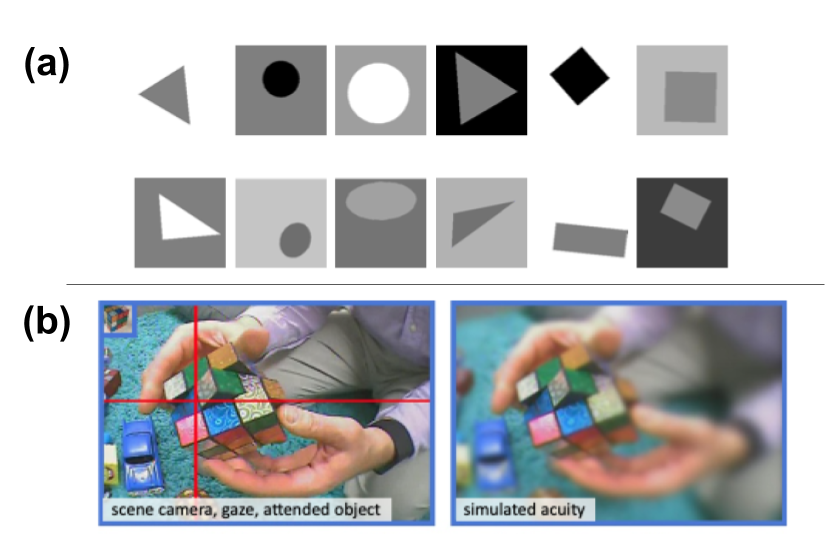
\includegraphics[scale=.4]{figures/curricula.png}
    \caption{}
        \begin{enumerate}[label=(\alph*)]
            \item Example of the simple (top row) and more complex (bottom row) shapes used for the curriculum in \textcite{bengio2009curriculum}. Taken directly from \textcite{bengio2009curriculum}. 
            \item Example of stimuli modified to be closer to the fovea-centric acuity of humans, used by \textcite{bambach2018toddler} to train a CNN. Taken from \textcite{bambach2018toddler}.
        \end{enumerate}
    \label{fig:curricula}
\end{figure} 


In addition to providing important insights on how to reduce the resource load required to train CNNs, \textcite{bambach2018toddler}'s work suggests that the appropriate environmental exposure might play an important role in producing an adequate model of human vision (as opposed to just model framework or architecture alone). Moreover, the empirical failures of CNNs at capturing object-centric visual phenomena seem less surprising given the discrepancies between the learning environment of CNNs and humans during development. In addition to the discrepancies highlighted by \textcite{bambach2018toddler}, CNNs also lack many important visual cues that are arguably pivotal to the inference of 3D shape from a 2D sensory input (e.g, optic flow, binocular viewpoints, etc). Future work investigating the plausibility of CNNs as models of shape perception might benefit from providing CNNs access to important visual cues that support 3D inference.

\subsection{Exploring Different Training Objectives}

Another important discrepancy between CNNs and humans is the various learning objectives both are trying to accomplish. The training objective of CNNs typically leveraged in the existing comparative literature is classification of single image categories. In contrast, the learning objective of human agents is arguably much more rich and multifaceted. That is, there are many important objectives a human must accomplish beyond object classification, such as spatial navigation, object tracking, communication, and object manipulation. Accordingly, many image statistics that might be useful for classification (e.g., background image textures) might be completely useless for other objectives like object manipulation. One hypothesis is that object-centric vision in CNNs or other deep learning models might require task-objectives where object-centric representations are useful. One difficulty is that CNNs trained via backpropagation require differentiable training objectives, which is difficult in unstructured environments. However, reinforcement learning paradigms (\cite{mnih2015human}) have been relatively successful at optimizing deep learning models for accomplishing non-differentiable learning objectives (such as, winning a game of Go; \cite{silver2016mastering}, and open up a richer exploratory space for future comparative studies.

\paragraph{Self-Supervision}\mbox{} \\

While reinforcement learning provides an avenue for testing the impact of more realistic learning objectives, it typically requires an unrealistic amount of training exposure and computational resources (\cite{lake2017building}). While standard backpropagation might be more efficient, it still typically requires large datasets of images \emph{labeled by human observers}. A practical alternative is to abandon the reliance on category labels. One technique is to leverage unsupervised learning, where models are tasked with capturing the statistical patterns embedded in a dataset \emph{independent of} any information about class-membership. Another recently emerging technique is \emph{self-supervised learning}, which tasks networks with performing diverse types of computationally tractable behaviors from unlabeled data (\cite{jing2020self}). For example, a network might be asked to correctly infer the color properties of a greyscale image (\cite{zhang2016colorful}), or determine the correct ordering a shuffled image (\cite{noroozi2016unsupervised}; figure \ref{fig:selfsupervised}). If the human perceptual system (a) exhibits the computational mechanisms required for image perturbation, and (b) has access to correct objective signals (either implicitly or via interaction with the environment\footnote{For example, interacting with and rotating an object in space might provide a self-supervised feedback signal about object shape, by comparing representational predictions with sensory data of subsequent visual events.}), then it seems plausible that humans \emph{could} leverage self-supervision when building perceptual representations\footnote{whether or not they actually do is an open question \\}. One candidate self-supervised learning objective in humans is building 3D visual representations from a 2D visual input\footnote{This objective could be realized in a CNN via transposed convolutions (\cite{dumoulin2016guide}) that map 2D inputs to 3D feature maps. \\}.

\begin{figure}[!h]
    \centering
    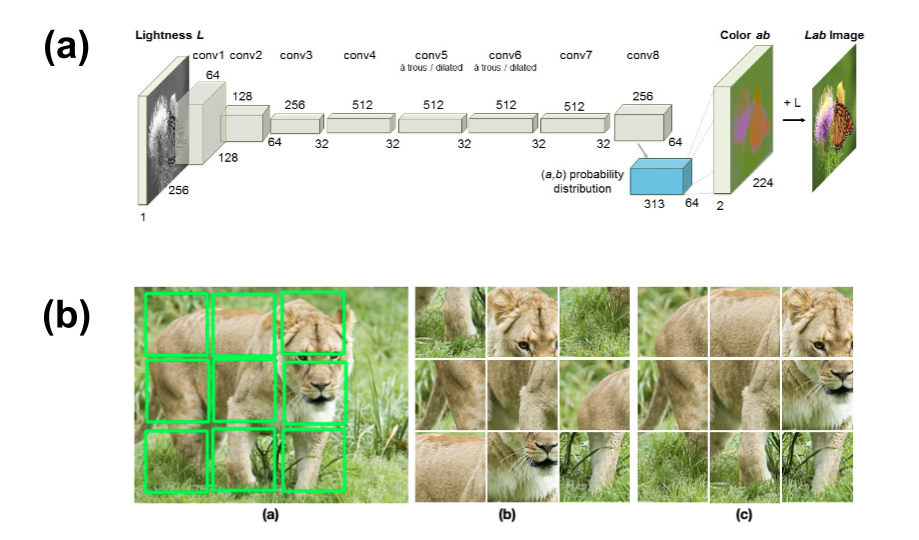
\includegraphics[scale=.4]{figures/selfsupervised.png}
    \caption{}
        \begin{enumerate}[label=(\alph*)]
            \item Self-supervised training objective that tasks the model with reconstructing a color image from a black and white image; taken directly from \textcite{zhang2016colorful}. 
            \item Self-supervised training objective where the model must correctly organize the blocks of a scrambled image; taken directly from \textcite{noroozi2016unsupervised}.
        \end{enumerate}
    \label{fig:selfsupervised}
\end{figure} 

\subsection{Adapting the Convolutional Operation}

Weight sharing (i.e., the reuse of synapses and the statistical knowledge they represent) is a key advantage of the convolutional operation: a limited set of parameters can be leveraged to capture local, translation-invariant patterns in a visual scene. In a standard convolution, this happens by tiling a window of parameters (i.e., feature detectors) across an entire image (figure \ref{fig:forwardOperations}). While this has been useful for computer vision, it requires that each feature detector be applied to all regions of a scene. In other words, feature detectors lack an intuitively useful characteristic of vision: selective attention. Recall that \textcite{kummerer2014deep} found that a pre-trained CNN could capture saliency maps of natural images (i.e., locations humans fixate on during viewing). While this information might be valuable for scene perception, CNNs have no mechanism for integrating it into their standard computations. 

This was a motivating factor for \textcite{mnih2014recurrent}, who allowed a recurrent network to leverage a reinforcement-optimized \emph{glimpse network} to sequentially sample local patches from an image during classification (unlike a CNN, which extracts local patches across the entire image)\footnote{This work followed up on previous successful attempts to give recurrent networks saccadic sampling actions similar to the ballistic eye movements of animals (\cite{schmidhuber1991learning,stollenga2014deep}). \\}. In addition to outperforming CNNs on variants of the MNIST dataset (\cite{lecun2010mnist}), \textcite{mnih2014recurrent} found that their network (dubbed \emph{recurrent attention model}; or RAM) was able to learn procedural actions that helped reduce attention to clutter in an image (figure \ref{fig:RAM}). It's intuitive to see how a selective attention mechanism (as leveraged by \cite{mnih2014recurrent}) could absolve \emph{some} of the comparative limitations of deep learning models --- such as the inability to generalize when objects are placed in unfamiliar contexts (\cite{rosenfeld2018elephant}), or the sensitivity to irrelevant, surface-level image statistics (\cite{jo2017measuring}). 

\begin{figure}[!h]
    \centering
    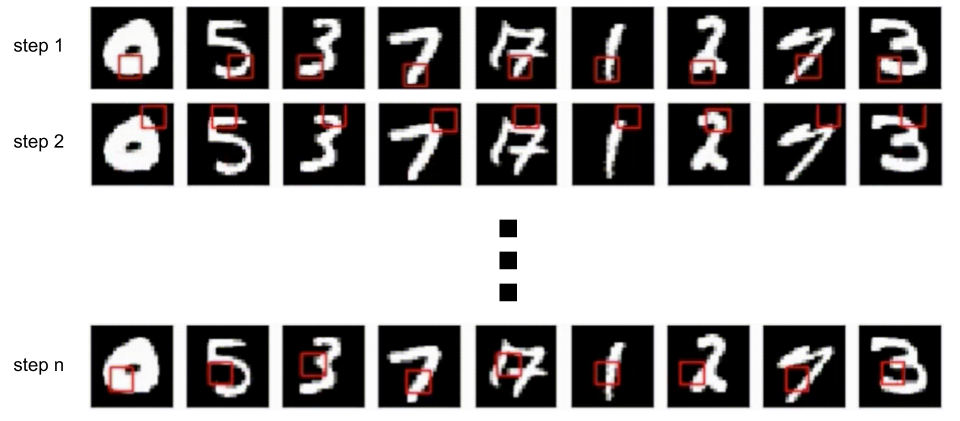
\includegraphics[scale=.4]{figures/RAM.png}
    \caption{Example of a recurrent attention model's selected regions of interest across 3 time steps. Adapted from \href{https://github.com/kevinzakka/recurrent-visual-attention}{Kevin Zakka's implementation}.}
    \label{fig:RAM}
\end{figure} 

Yet another discrepancy between CNN training and human perception is that CNNs lack the mechanisms necessary to leverage temporal information in visual scenes (i.e., any form of memory). This seems critically important given that humans experience visual information as a temporal sequence of events, rather than a random assortment of unrelated snapshots. Additionally, how an object moves through space may provide critical statistical details that could be leveraged for object-centric computations. Recurrent networks are deep learning models that can leverage a hidden state from previous timesteps in a sequential learning task (\cite{schmidhuber2015deepSchol}). Convolutional layers can be naturally integrated with a recurrent hidden state to process frame sequences in a video rather than a single, motionless image; in fact, they've already been leveraged for video classification problems with state-of-the-art success (\cite{yue2015beyond,xu2016recurrent})\footnote{This allows CNNs to learn features that involve motion through time (\cite{xu2016recurrent}).}. An additional useful property of recurrent networks is their ability to approximate programmatic solutions to learning problems (\cite{schmidhuber2015deepSchol}), which might endow CNNs with the ability to perform the perceptual reasoning (which they currently lack; \cite{gulccehre2016knowledge,fleuret2011comparing}).

\paragraph{Capsule Networks}\mbox{} \\

The discrepancies discuss thus far in this section caution against making strong conclusions from existing studies comparing humans and deep learning models, particularly in regard to the question of whether the convolutional operation could produce practical, object-centric visual representations. While the discussed extensions (psychologically inspired perceptual curricula, self-supervised learning objectives and reinforcement learning, selective attention and recurrent memory) might get deep learning models closer to object-centric perception, it may be the case that the convolutional operation alone is not enough\footnote{It may have been unreasonable for any researcher to assume that a half-century old discovery (deep convolutional networks) could adequately solve one of psychology's most difficult explanatory challenges (the binding problem; \cite{roskies1999binding}) \\}. Some researchers have proposed the need for an entirely new computation that directly models the spatial relationships between features in the visual heirarchy (\cite{hinton2011transforming,sabour2017dynamic}).

One such alternative computation was proposed by \textcite{hinton2011transforming}, who described a novel computational operation on sets of neurons referred to as ``capsules''. Rather than relying solely on information about pixel intensities from a retinal image, \emph{capsule networks} are given nonvisual information relating to how an image has been transformed (e.g., rotated, scaled, translated, etc), which may provide important information about the relationships between visual features. Importantly, capsule networks were designed to produce representations that are \emph{equivariant} to image transformations, as opposed to \emph{invariant} to image transformations\endnote{An invariant representation is a representation that is consistent even when an incoming stimulus is modified in some way. For example, CNNs produce classification responses that are typically \emph{invariant} to translation (e.g., moving a visual feature from one region to another). \emph{Equivariance} refers to representations that change \emph{with} modifications to an image. For example, if an object is rotated in 3D space, an \emph{equivariant} representation should experience some corresponding change of similar, scaled magnitude. \\}. Because the capsule layer is differentiable, capsule networks retain the critically important end-to-end properties of connectionist models. Capsule networks deviate from traditional models of vision in that they leverage non-visual information (i.e., values representing the scale of image transformations) during visual computations. Interestingly, it seems psychologically reasonable that the human mind could leverage knowledge of visual transformations as well\footnote{For example, binocular visual inputs could provide information about spatial rotation (i.e., using the difference in visual angle between the left and right eye). \\}.


\subsection{Leveraging Structured Representations}

Graphical structure (either as propositional logic or as graphical models) has been frequently invoked in many areas of cognition, including, language (\cite{vitevitch2008can}), semantic knowledge (\cite{quillian1967word,collins1975spreading}), analogical reasoning (\cite{gentner1983structure}), and perception (\cite{pylyshyn1973mind,biederman1987recognition,hummel1992dynamic}). Structured graphical models have also been pivotal in theories of causal cognition (\cite{danks2014unifying}). While graphical models can be composed of random variables of any kind, the variables that are particularly important for understanding our perceptual environment intuitively seem to be objects and their interactions. Consequently, any adequate model of end-to-end cognition should provide an explanation of \textbf{(a)} the role of structured representations in perception and cognition, and \textbf{(b)} how perceptual variables can be mapped to components of a structured representation.  

Variational inference provides a method for training deep learning models to produce structured, probabilistic models from unstructured data (\cite{kingma2013auto,johnson2016composing}), which has been an otherwise historically difficult task (\cite{hinton1981shape,hummel2004solution}). There are a number of reasons why this is a particularly attractive feature for an end-to-end cognitive model of human perception and cognition. For instance,  graphical structure is commonly invoked in theories across many various branches of psychology (\cite{quillian1967word,collins1975spreading,vitevitch2008can,biederman1987recognition,danks2014unifying}); integrating them with deep learning models might alleviate some of the explanatory failures in the existing comparative literature. In addition --- as stated earlier --- structure in our perceptual environment often reflects objects and how they interact; regularizing structure in the hidden layer of deep learning models might induce pressures to represent data in a object-centric manner. Further, graphical models provide a medium for a shared representational language, which might provide a preliminary explanation of how human beings can make analogies and causal inferences across vastly different perceptual and conceptual domains. Finally, leveraging graphical structure in deep learning networks may provide a constrained bridge between the historically divided theories of perception and theories of symbolic cognition (\cite{goldstone1998reuniting}).


% - - - - - - - - - - - - - - - - - - - - - - - - - -


\section{Conclusions}


% summary: they cant do the formidable binging problem


Deep learning models (specifically, CNNs) have provided powerful accounts of a number of physiological (\cite{yamins2016using,kietzmann2018deep}) and behavioral (\cite{lake2015deep,peterson2016adapting,kummerer2014deep}) phenomena, despite being fundamentally limited in their ability to form object-centric representations (\cite{baker2018deep}) and perform visual reasoning tasks (\cite{stabinger201625}). However, modeling human perception with CNNs is a relatively recent research endeavor. As noted in the previous section, there are many recent advancements in the deep learning literature that have yet to be integrated into comparative modeling studies. There are various extensions to the perceptual curricula (\cite{smith2018developing,bengio2009curriculum}) and task objectives (\cite{jing2020self}) of CNNs that may provide promising avenues towards the goal of modeling psychologically realistic, object-centric visual representations from unstructured perceptual data entirely. Further, various extensions to the standard operations of connectionist networks may provide a powerful mechanism for representing spatial relationships between object parts (\cite{hinton2011transforming,sabour2017dynamic}) and mapping perceptual components onto structured graphical representations (\cite{kingma2013auto,johnson2016composing}), while retaining the theoretically attractive properties of end-to-end optimization with a relatively universal learning algorithm in a brain-style network.

\theendnotes

% - - - - - - - - - - - - - - - - - - - - - 
% - - - - - - - - - - - - - - - - - - - - - 


% % % % % % % % % %
%
%   REFERENCES
%
% % % % % % % % % %

\pagebreak
\pagestyle{empty}
\renewcommand\bibname{References}
\printbibliography

% - - - - - - - - - - - - - - - - - - - - - 
% - - - - - - - - - - - - - - - - - - - - - 

\end{document}
